\documentclass[10pt,conference,compsocconf]{IEEEtran}

\usepackage{amsmath, relsize, amsthm, amssymb, amsfonts}
\usepackage{cite}
\usepackage{float}
\usepackage{graphicx}
\usepackage{hyperref}
\usepackage{listings}

\graphicspath{{img/}}

\begin{document}
\title{Machine Learning - Road Segmentation}

\author{
  Julien Niklas Heitmann
  \and
  Philipp Khlebnikov
  \and
  Louis Gabriel Jean Landelle
} 

\maketitle

\begin{abstract}
The goal of this project is to segment roads in aerial satellite images, i.e. to assign a label to each pixel (road=1, background=0). We use convolutional neural network  with rectified linear unit (ReLU) as activation function and maxpooling to develop the classifier as it has proved its good performance in image segmentation. More specifically we will use a U-Net, a more recent technique based on CNN, which is sometimes referred to as a "fully convolutional neural network", because its output is a 2D matrix of approximately same height and width as the input image, depending on whether or not border pixels are lost during convolutions. 
\end{abstract}

\section{Introduction}

Image segmentation is a technique that is becoming increasingly used in computer vision for different purposes. In medical imaging, image segmentation has proven its utility to identify tumours, osteoarthritis on a radiography. More recently, with autonomous cars, this became even more useful as the car has to identify danger and road signalisation instantly, continuously and precisely. Moreover the number of images that have to be analysed per second is high, hence the methods must be accurate and fast.

With the increasing performance of computers and powerful parallelization capabilities of GPUs, advanced machine learning techniques have been developed to predict or classify elements. Open source libraries, such as Tensorflow or Theano, have been developed to help people to easily implements neural networks.

The aim of this project is to classify pixels of 50 aerial images into two categories: road and background (i.e buildings, parking lots, fields water...). In addition to that 100 aerial images were provided with their groundtruth labels to train the model.

The most commonly method in image segmentation is the convolutional neural network (CNN) as it has proven its efficiency in that kind of tasks and as the other simpler techniques can not extract enough information from pictures. The CNN can also take into account the morphology of the picture, and we will see that it is an important task for our problem.

After some mathematical formulation on the $F_1$ score and the problem we are going to perform some exploratory data analysis to better understand the structure of the data and the complication that we can have. After what we are going to explain our base model and the U-Net model structure that we mainly used.

\begin{figure}
    \centering
    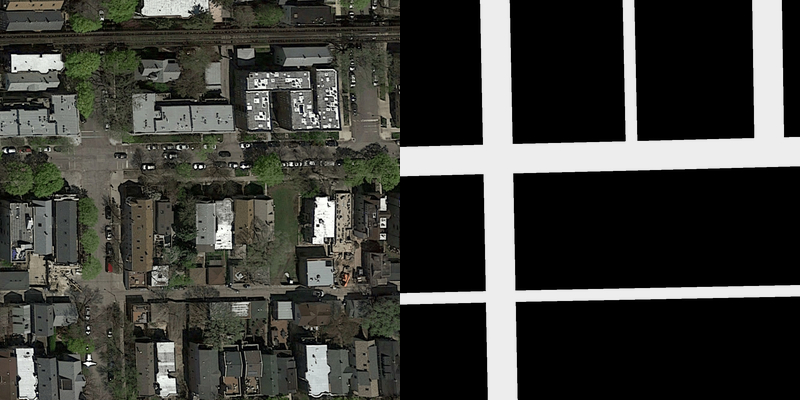
\includegraphics[scale=0.30]{combined.jpg}
    \caption{Area from training set and the corresponding ground truth}
    \label{fig:overlay}
\end{figure}

\section{Problem Formulation}
Let $S$ and $R$ be respectively the set of aerial images and the corresponding set of road map images. We define $R(i,j)=1$ if the corresponding pixel in location $(i,j)$ in $S$ is a road and $R(i,j)=0$ otherwise. In this project we want to find $p(R(i,j)|S)$.\\

To find the most accurate prediction for $p(R(i,j)|S)$ the simple machine learning techniques were no more sufficient, thus we had to use more complex techniques such as convolutional neural networks (CNN).

The performance of the classification is evaluated using the $F_1$ score, which is defined as follows:
$$ F_1=\frac{2\cdot precision \cdot recall}{precision + recall}$$
The $F_1$ score is in range $[0,1]$ and the closer it is to 1 the better the model predicts.

\section{Exploratory data analysis}
The training data set is composed of 100 aerial images and 100 corresponding groundtruth images,of size $400\times400$. Each pixel of the aerial images is coloured, thus is of dimension 3 in a range from 0 to 255 for red, green and blue. Each pixel of the road map images is of dimension 1 taking value 1 if the pixel corresponds to a road and 0 otherwise. The test data set is composed of 50 aerial images each of them of size $608\times608$ coloured pixels. At first glance, it seems like all images were taken at the same height, hence test images correspond to larger areas, and not to a higher resolution as one might think. Moreover, it appears as if theses pictures were taken in the same geographical area or in same country (probably the US), as some common architectural features can be identified in all of them. \\

The goal is to classify blocks of 16 $\times$ 16 pixels, considering that we classify each block as follows:

\[
\begin{cases}
    1, & \text{if } \frac{1}{256}\sum\limits^{16}_{i,j=1}p_{i,j} \geq 0.25\\
    0, & \text{otherwise}
\end{cases}
\]

Looking on the data set we see that the classification will be difficult and that can not be performs using only information of the pixel, i.e its colour. As shown in the Figure \ref{fig:overlay}, according to the ground truth, some tree parts, in green, are classified as road, while parking lots, in grey, are classified as background. 

Hence it is reasonable to think that the classifier has to take in consideration the context of the pixel and use information from neighbour pixels.

\section{Models and method}

\subsection{Baseline}

This is the provided baseline for the EPFL machine learning project on road segmentation. It consists of a CNN with two convolutional+pooling layers, with soft-max loss. The performance is poor, and the model is not fit for such a complex segmentation task. Limitations include an inability to understand the context of pixels, which is important for correlations such as : cars are present on roads, houses roofs are aligned to roads, etc. The $16\times16$ patch predictions are to be predicted from individual pixels predictions. We overcome those limitations changing the model, using a U-Net.

We use a more complex model, the U-Net, as described in the U-net section. The U-Net is not the solution of all problems however, we describe in this section our incremental improvements, that are quantified in the section Final Results.

\subsection{Scale rectification}

The training images are $400\times400$ pixels, and the testing images are $608\times608$ images. However, this is not just a rescaling, as if we compare the scales of houses, roads, cars, we notice that the larger images are in fact a larger area taken from a similar "camera height", and downsampling the testing images, our first approach, yielded poor results. We found an alternative that would conserve this "camera height" of the training images, by using \textit{four split} cropping : each $608\times608$ is split into four $400\times400$ sub-images corresponding to each corner, thus overlapping in some area, that we individualy predict. The predictions are then aggregated using a method such as the mean of overlapping predictions, or the maximum prediction choice. This yields a large $F_1$ score improvement.

\subsection{Dataset augmentation} \label{sub:aug}

The training images are similar in a way that most roads are axis-aligned, with just a few diagonal/titled roads. Unsurprisingly, the predictions works better on axis-aligned roads compared to diagonal/titled roads. We solve this problem using Keras' ImageDataGenerator, which is able to augment the training dataset using transformations. We use the \verb|rotation_range| parameter to perform a randomized rotation, tilting the axis-aligned roads. \verb|fill_mode='mirrored'| is used to fill in the missing pixels resulting from the rotation, which produces natural-looking continuation of roads and buildings. This yields a moderate $F_1$ score improvement.

\subsection{Chosen validation set}

Because the validation metrics are a better monitoring choice, it is important to split the training set into a training and a validation separate dataset. Note that some images are very similar, with suburbs views with straight roads, providing poor information to the model. Some other images provide a more precious information, with the presence of curved roads, parks, water, and other such unconventional features. The few number of training images (100) means that the validation dataset could take away many "precious" images from the training set, we solve this problem using fixed, chosen train/validation sets. This is activated via a flag, \verb|-cv|, and this resulted in an increase of performance (see Final Results).

\section{U-Net}
The U-Net \cite{DBLP:journals/corr/RonnebergerFB15} is a CNN that can extract from a small data set a lot of information. It was developed by the University of Freiburg in Germany for data segmentation and image recognition. 

As shown on Figure \ref{fig:Unet}, the U-Net derives its name from a graphical representation of its layers, the two branches of the U being the convolution and the deconvolution halves. The model was created using the Keras library on a Tensorflow back-end. The first half of the U is stacking multiple "units" each of 2 Conv2D layers followed by 1 MaxPooling2D layer, with 2 Dropout layers at the base of the U, and the second half of the U is mirroring each unit with Concatenate layers in-lieu of MaxPooling layers, i.e 1 Concatenate layer followed by 2 Conv2D layers. As the information flows from the Input layer to the output layer, each channel represents more complex information about our image, as is with the convolutional style of neural networks - the first layers might represent features such as a simple edge extraction, color aggregation of neighbouring pixels, where later layers might represent complex properties such as connectivity with other roads, presence of cars, neighbouring houses, etc.

The specificity of the U-Net architecture comes the process of convolution/deconvolution which enables an image of size $N \times N$ to be transformed into another image of the same $N \times N$ size, using complex properties. This is well adapted for an image segmentation problem, where we want a resulting image of the same size with pixel colors representing the probability of the corresponding input pixel to belong to a class.

\subsection{Conv2D}
The Conv2D layer performs spatial convolution. We use 64 filters on the first convolution layer, and double the filters amount each subsequent convolution layer. We use a convolution kernel of size $3\times3$. It is its minimum size, minimising the amount of weights in each Conv2D layer, the successive convolutions/maxpooling making up for this loss of context resulting from this small size. We used the rectified linear unit function (ReLU) as activation function, defined by $f(x)=max(0,x)$. It has several advantages such as having a small computation cost, better gradient propagation but is not differentiable at 0 and is unbounded. Nevertheless, it has proven its good performance in image-based neural networks, hence we decided to use it.

\subsection{MaxPooling2D}
The MaxPooling2D layer performs spatial max-pooling. We use a pool\_size of $2\times2$ thus it halves the image size. This layer aggregates information of multiple convolution results, while reducing the amount of weights we would get from a naive Conv2D-only stack of layers.

\subsection{Dropout}
Two Dropout layers are used before and after the last 2 convolutions of the first half of the U shape, with a rate of 0.5 (proportion of input units being set to 0) forcing the usage of potentially previously ignored weights. This should prevent overfitting. 

\subsection{Optimizer and loss}
The model uses the Adam stochastic optimisation method, using the Keras implementation, following the description from the original paper \cite{Ruder2016AnOO}, using a learning rate of $1\cdot10^{-4}$. 

The segmentation problem is not a multiclass problem (the number of class $M = 2$). Thus we use the loss method of binary-crossentropy instead of categorical-crossentropy:

$$\sum_{i}-(y_i \cdot log(p_i) + (1 - y_i) \cdot log(1 - p_i))$$

with : 
\begin{itemize}
    \item $y_i$ : the actual label of the ith pixel
    \item $p_i$ : predicted probability of class 1
\end{itemize}

This results in a neural net with 31,032,837 trainable parameters for our best model.

\begin{figure}
    \centering
    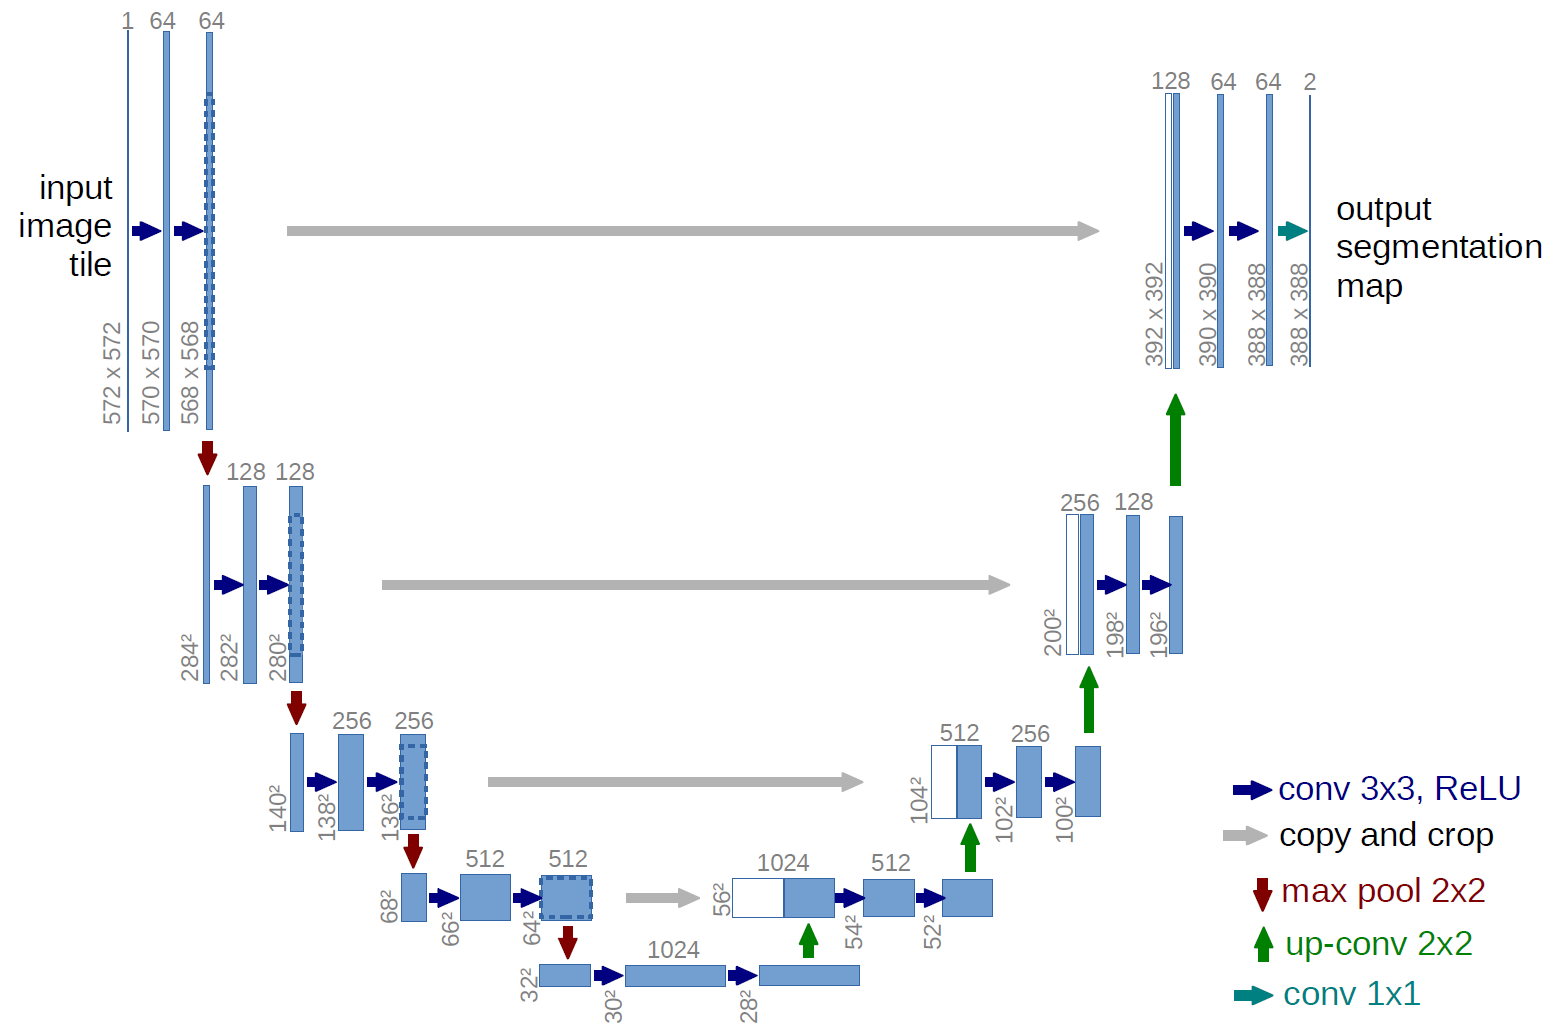
\includegraphics[scale=0.15]{u-net.png}
    \caption{U-Net architecture}
    \label{fig:Unet}
\end{figure}

\section{Implementation details and training}

\subsection{Code architecture}

The project code is structured as follows:
\begin{itemize}
\item \verb|common.py| : contains all of our constants, most of them used throughout the other scripts
\item \verb|model.py| : the keras model of the U-Net neural network
\item \verb|preprocessing.py| : functions used for dataset extraction and preparation
\item \verb|postprocessing.py| : functions used for results images, csvs, generation, aggregation, etc.
\item \verb|setup_env.py| : functions used for automatic creation and checking of the folders needed
\item \verb|utrain.py| : script executing the logic for training, which can either be imported and used via its main() function or directly launched in terminal (see help via \verb|python utrain.py -h|). This script is responsible for the generation of the hdf5 checkpoint files, and the csv/graph images logging the metrics evolutions
\item \verb|utest.py| : script executing the logic for testing, which can either be imported and used via its main() function or directly launched in terminal (see help via \verb|python utest.py -h|). This script is responsible for the generation of the masks images, optionally the logits and the overlay files, and the csv submission files.
\end{itemize}
More information in \verb|README.md|.

\subsection{GPU Acceleration}

\subsubsection{Local training}
We had access to a single NVIDIA GTX 1070 Ti GPU, which we used for training using the tensorflow-gpu backend with Keras. This kind of GPU performed 1000 epochs in about 3h to train our best model, \textit{Unet zeta}

\subsubsection{Google Colab}
Part of our training was performed on the Google Colab GPU runtime. It is free, and considerably faster than our CPUs. We uploaded our scripts to Google drive, mounted the drive inside Colab, imported utrain and launched it from there. The Google Colab runtime performs a little bit slower than the GTX 1070 Ti, but can be used to train multiple models in parallel, provided you create multiple accounts.

\section{Final results}

\noindent
\textbf{Model parameters:} all models were trained for \textbf{100} epochs, with \textbf{80} training steps per epoch, hence \textbf{20} validation steps per epoch (validation images either stay the same during the entire training, or can be generated "on the fly" given an initial validation split and a fixed set of allowed image transformation, such as rotation, horizontal/vertical flips, etc.), and a batch size of \textbf{2}. For the U-Nets, out of the 100 epochs, we keep the model checkpoint that achieved the best validation accuracy. Except for \textit{Unet epsilon}, the first layer of the Unet processes grayscale $256 \times 256$ images. Note that we left out an additional model, call it \textit{Unet gamma}, that trains using the original (but grayscale) images, that means no downscaling is done before feeding the images to the first layer of our neural network. This is because it did not perform better than our current best model, \textit{Unet zeta}, and took significantly longer to train (having more trainable parameters). Similarly, \textit{Unet epsilon} also has more trainable parameters, because it trains on $256 \times 256$ RGB images, that come with 3 instead of 1 input channels. 

In addition to the $F_1$ CrowdAI metric, we implemented a way to evaluate our own "internal" $F_1$ score by predicting the training dataset. Because of overfitting possibilities, this $F_1$ score risks being higher than the true $F_1$ score, nevertheless, because of the Dropout layers, we can hope that the overfitting is low enough for the Train $F_1$ score to be a good proxy for the analysis of the difference between our models for the CrowdAI $F_1$ score.

\begin{table}[H]
    \begin{center}
    \scalebox{0.9} {
    \begin{tabular}{c|c|c|c|c|c|c}
        Model & Unet & Agg & Aug & Chosen Val & Train $F_1$ & CrowdAI $F_1$ \\ \hline
        Tf aerial & - & - & - & - & 0.66 & 0.43 \\
        Unet alpha & \checkmark & - & - & - & 0.93 & 0.59 \\
        Unet beta & \checkmark  & Mean & - & - & 0.93 & 0.80 \\
        Unet delta & \checkmark & Max & \checkmark & - & 0.94 & 0.884 \\
        Unet epsilon & \checkmark & Max & \checkmark & - & 0.92 & 0.86 \\
        Unet zeta & \checkmark & Max & \checkmark & \checkmark & 0.95 & 0.888 \\
        \end{tabular}
    }
    \end{center}
    
    \caption {$F_1$ values by model} \label{tab:title} 
\end{table}

\begin{figure}
    \centering
    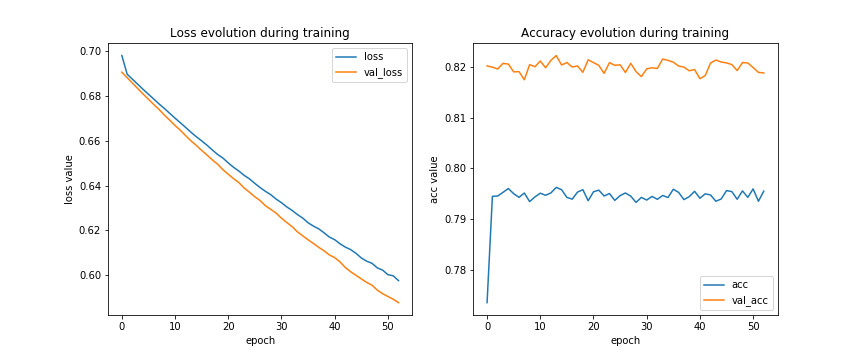
\includegraphics[scale=0.32]{seed_plateau.jpeg}
    \caption{Training with a bad seed}
    \label{fig:seed}
\end{figure}

\begin{figure}
    \centering
    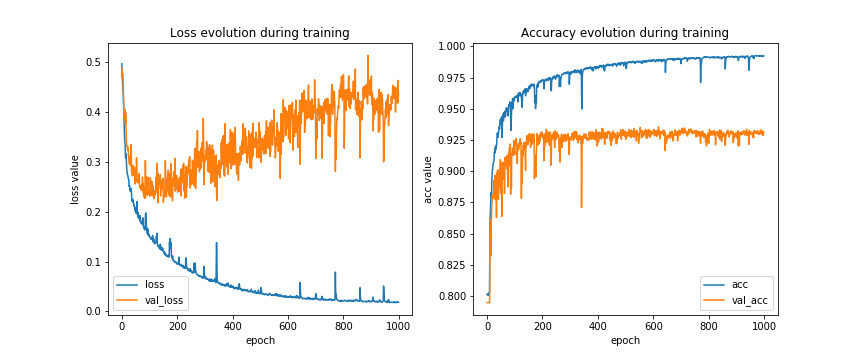
\includegraphics[scale=0.32]{best_model.jpeg}
    \caption{\textit{Unet zeta} metrics evolution}
    \label{fig:best-model}
\end{figure}

\begin{figure}
    \centering
    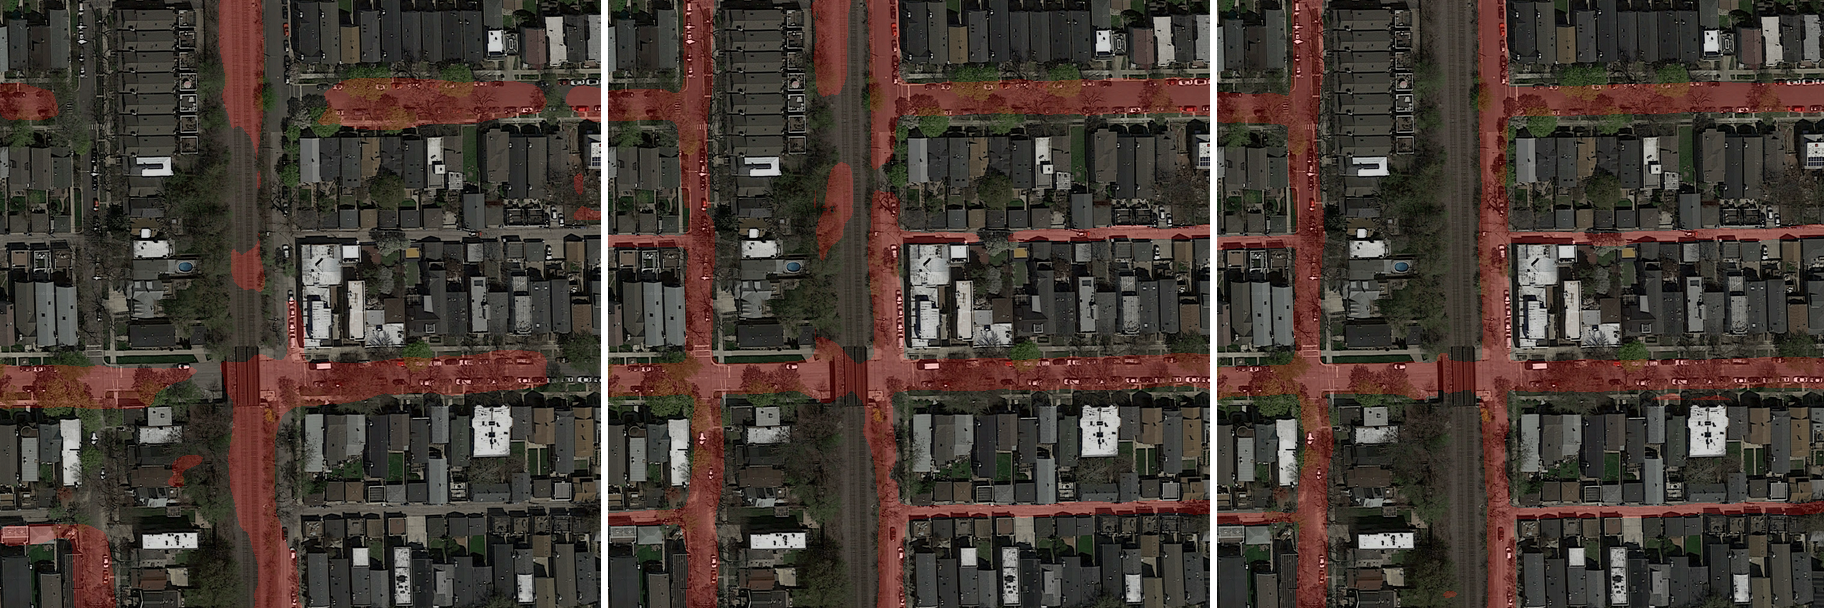
\includegraphics[scale=0.17]{improvement.png}
    \caption{Evolution of overlays}
    \label{fig:overlays}
\end{figure}

\begin{figure}
    \centering
    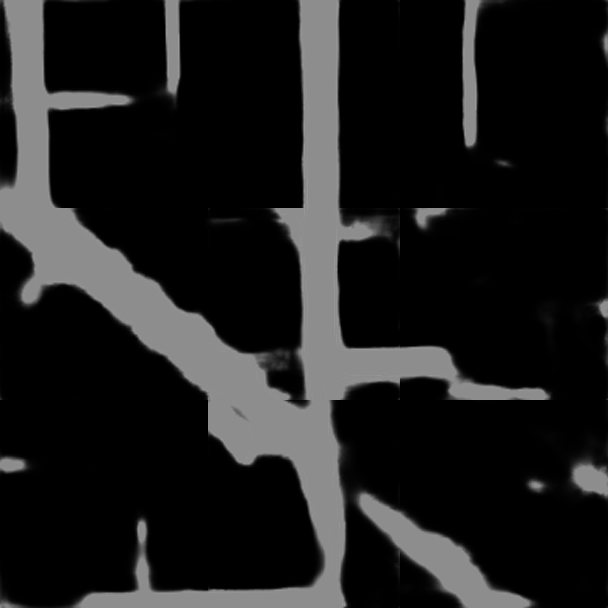
\includegraphics[scale=0.20]{logit_049.png}
    \caption{Issue with combining split predictions}
    \label{fig:four-split}
\end{figure}

\section{Discussion and future work}
Our best model was able to outperform by a very large margin the baseline model. It was also able to place high in the leaderboard of the CrowdAI competition. Some problems reside, such as the problematic randomness that appears to stay even after a thorough elimination of all randomness sources we could find using a common, global seed. Sometimes, the training will appear to find an equilibrium and be stuck there for indefinite periods of time, never improving on the first epoch as shown on Figure \ref{fig:seed}. If this problem occurs even after using common.SEED = 2018 and 1227, one can download an hdf5 at https://uploadfiles.io/xcpjk and run \verb|utest.py| on those. Augmenting the training dataset is an option, as we consider 100 to be a low number of training images. Finding more interesting road structures could also positively impact the training. The \textit{four split} method is producing subtle frontiers between overlap areas \ref{fig:four-split}, which is normal and might be eliminated via image smoothing algorithms. ZCA whitening could be a possible improvement. Finally, the architecture described in \cite{DBLP:journals/corr/RonnebergerFB15} does not make use of padding (for convolution), hence the output mask only predicts a centred area of the input image. Increasing the input image size with \textit{mirroring} as described in \ref{sub:aug} might result in better predictions of border pixels. The time limit prevented us from trying those leads.

\bibliography{bibl}{}
\bibliographystyle{ieeetr}
\end{document}
